\documentclass[journal]{vgtc}                % final (journal style)

\ifpdf%                                % if we use pdflatex
  \pdfoutput=1\relax                   % create PDFs from pdfLaTeX
  \pdfcompresslevel=9                  % PDF Compression
  \pdfoptionpdfminorversion=7          % create PDF 1.7
  \ExecuteOptions{pdftex}
  \usepackage{graphicx}                % allow us to embed graphics files
  \DeclareGraphicsExtensions{.pdf,.png,.jpg,.jpeg} % for pdflatex we expect .pdf, .png, or .jpg files
\else%                                 % else we use pure latex
  \ExecuteOptions{dvips}
  \usepackage{graphicx}                % allow us to embed graphics files
  \DeclareGraphicsExtensions{.eps}     % for pure latex we expect eps files
\fi%

%% it is recomended to use ``\autoref{sec:bla}'' instead of ``Fig.~\ref{sec:bla}''
\graphicspath{{figures/}{pictures/}{images/}{./}} % where to search for the images

\usepackage{microtype}                 % use micro-typography (slightly more compact, better to read)
\PassOptionsToPackage{warn}{textcomp}  % to address font issues with \textrightarrow
\usepackage{textcomp}                  % use better special symbols
\usepackage{mathptmx}                  % use matching math font
\usepackage{times}                     % we use Times as the main font
\renewcommand*\ttdefault{txtt}         % a nicer typewriter font
\usepackage{cite}                      % needed to automatically sort the references
\usepackage{tabu}                      % only used for the table example
\usepackage{booktabs}                  % only used for the table example

\onlineid{0}

\vgtccategory{Research}

\vgtcpapertype{system}

%% Paper title.
\title{Decision Support for Organizational Change (DSOC)}

\author{Rob Barwell and Eric Spero}
\authorfooter{
%% insert punctuation at end of each item
\item
 Rob Barwell and Eric Spero are with Carleton University. E-mail: robert.barwell/eric.spero@carleton.ca.
}

%other entries to be set up for journal
\shortauthortitle{Biv \MakeLowercase{\textit{et al.}}: Global Illumination for Fun and Profit}
%\shortauthortitle{Firstauthor \MakeLowercase{\textit{et al.}}: Paper Title}

\abstract{
  Our abstract goes here.
} 
\keywords{Organizational change, decision-making, information visualization}

%% ACM Computing Classification System (CCS). 
%% See <http://www.acm.org/class/1998/> for details.
%% The ``\CCScat'' command takes four arguments.

\CCScatlist{ % not used in journal version
 \CCScat{K.6.1}{Management of Computing and Information Systems}%
{Project and People Management}{Life Cycle};
 \CCScat{K.7.m}{The Computing Profession}{Miscellaneous}{Ethics}
}

%% Uncomment below to include a teaser figure.
\teaser{
  \centering
  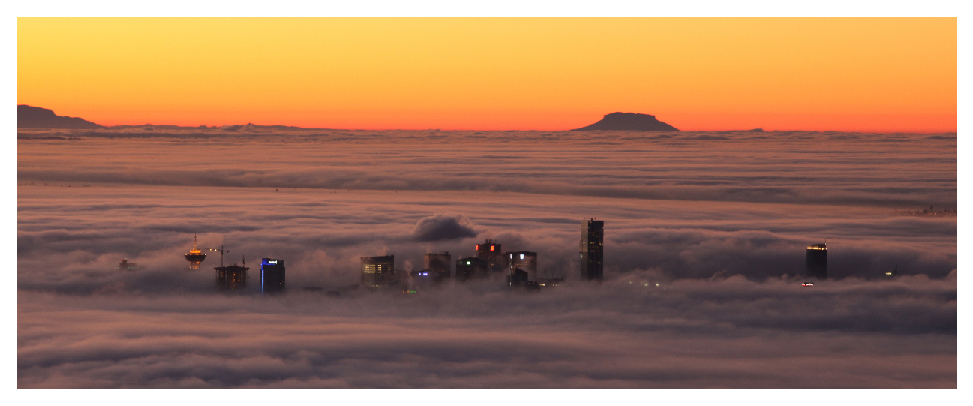
\includegraphics[width=\linewidth]{CypressView}
  \caption{In the Clouds: Vancouver from Cypress Mountain. Note that the teaser may not be wider than the abstract block.}
	\label{fig:teaser}
}

%% Uncomment below to disable the manuscript note
\renewcommand{\manuscriptnotetxt}{}

%% Copyright space is enabled by default as required by guidelines.
%% It is disabled by the 'review' option or via the following command:
%\nocopyrightspace

\vgtcinsertpkg

%% Start document!

\begin{document}

\firstsection{Introduction}

\maketitle
The idea of organizational change has started to shift over the past decade with the introduction of the gig economy and other non-traditional employment models.  Historically a person would obtain a job after high school and university and stay with the same company until retirement.  This has fundamentally changed where employees are commonly switching jobs every 2-3 years and some might be more contract workers then employees.  This can stress an organization especially if the change is not well understood.  Understanding the intricate interlocking contingencies between people in an organization can be difficult and changes to its social structure hard to understand.  This paper looks to create a visualization tool to help an organization understand these changes and help decision makers minimize negative side-effects from the change.
The visualization will support the other concept we want to introduce which is organizational change from the information flow perspective vice the traditional organization hierarchy.  To understand how change will disrupt the flow of information through an organization you first have to model the flow.  We have chosen to model the flow based on the email communications within an organization combined with social networking theory.

\section{Background}

\subsection{Problem Space}
Similar to the design aspect of the problem we also went through an iterative process to redefine our initial problem.  The original problem we started with was "How to address empty positions within an organization?"  This was a topic of interest to us as we know many organizations are facing organizational modeling problems within the current context of the "gig" economy where employees are constantly changing jobs and might only be with a company for a short term.  This leads to organizational charts that are quickly out of date and do not accurate reflect the true distribution and flow of work within an organization.  
After reflect this was further refined into the following problems:
\item “How do we support decision makers to minimize negative side-effects from organizational change?”
\item “How do we value a person in the organization?”
\item “How do we provide options to users to address vacancies within an organization?”
These can be further reshaped to what a user community (i.e. managers) would understand which are:
\item "Where is the gap?";
\item "How big is the gap?"; and
\item "What can I do about the gap?".

\subsection{Option Space}
With the problem space defined we can focus on how the user would explore the problem space.  This is typically done by viewing the problem from different angles or through different lens.  When we discussed our refined problem with users and asked them how they would address the problem they talked about exploring the problem by looking at it from an organizational perspective and a process perspective.  When we discussed how to fill the gaps we also noted a third perspective around redundancy.  Below is a quick description of the mental model for each view:
\item Organizational - 
\item Process - 
\item Redundancy - 

\section{Design}

Our visualization came organically through a couple iterations and discussions with real world users.  The original design was developed by the authors, this design was then presented to real world users interested in the topic.  Based on their feedback adjustments were made to refine the design.  After a second round a feedback from the users we showed it to academics who provided further feedback.  This resulted in the final design presented in this paper.

\subsection{Data}
To achieve the goal of a visualization to communicate knowledge or discover new knowledge we first had to develop a problem set to create a visualization for.  Our colleague Brad Mazurek came up with the original idea to understand the impact of information flow through an organization when the organization changes.  This resulted in a number of discussions to determine how to model information flow and visualize the impact to any changes within the flow.  The result of this discussion was using email and associated SMTP information as a representation of information flow within an organization.
Traditional organization structure is captured within an organizational chart, however these charts tend to be outdated quickly and do not represent the true flow of information or value of an individual employee.

The initial value model is based on a primitive concept of each email representing a value of 1.  This results in the generation of a node, representing a person, and an edge representing a single email between 2 people with a weight of 1.  Using SMTP header information this was easy to model in a database.  Alternative value models are discussed in section 5 under future work.

To demonstrate our value model we chose the popular Enron email data set.  This data set was originally made public during the Federal Energy Regulatory Commission investigation.  It contains the emails of approximately 150 users in the Eron organization.  Most of these users are senior managers.  This particular data set has been studied a number of times primarily with a focus in social networking and natural language processing.  This paper will use this data set to illustrate our visualization to support the flow of information through an organization.  

In addition to the email boxes of users we also required an organizational chart to represent what the organization thinks is the structure of the employees.  Unfortunately, during our research we were unable to obtain an organizational chart.  This is a well documented problem with the data set which has limited research against it for lack of undisputable verification.  Since our research is primarily focused on the visualization and not the under laying data we decided to use the organizational chart developed by A, B, C in the paper XYZ (https://event.cwi.nl/lsde/2015-2016/group5.pdf).  Based on our research this is one of the more accurate examples to model the organization from a standard organizational structure vice a social networking structure.

\subsection{Data Preparation}

The Enron data set was obtained from Carniege Mellon University.  It was processed using a Python script to parse all the SMTP header information from a given email.  This was then stored in a MySQL database for further processing by the application.  SMTP information was chosen since it contained all the information required to construct the nodes and edges within the graph.  

\subsection{Methodology}
Before conducting any design work we first needed to come up with a methodology to use and the supporting infrastructure and resources.  Based on a number of papers we reviewed on the topic such as "The Challenge of Information Visualization Evaluation" we had to think about our evaluation criteria and approach.  Based on some of the concepts presented in "Empirical Studies in Information Visualization: Seven Scenarios paper" we determined we needed an iterative approach similar to the approach presented in the paper of Pre-design, design, prototype, deployment, and re-design.  This approach involved gaining support for real world users and academics to provide informal feedback through the design process.  This also allowed us to strike a balance between modern visualization concepts that push the envelope and how a real world user would interpret those concepts.  By version 3 of our design we started to see the balance between the modern visualizations that the academics helped generate and the needs of real world users.  Our opinion is this approach should be standard in any visualization development to ensure there is a user adoption path that meets the needs of a broader audience.
After the initial design was explored we first presented it to real world users to validate our brain storming.  We obtained a lot of valuable feedback which we will guide you through in the next section.  The second design was then shown to academics to help generate creative solutions to some of the challenges real world users had identified but we were unable to solve on our own.  After this we conducted another review with users who noticed our design had evolved significantly since the first time they viewed it.

\section{Evolution of Design}

Designing a functional layout that conveyed the complex problem of organizational change turned out to be complex.  The initial part of the problem focused around the sense making problem that is described in the "Ivan Herman" paper.  We needed an intuitive design that would allow the user to quickly understand the different views into the problem and allow the user to quickly understand where they are in their mental process.

\subsection{Layout}
\subsubsection{Structure}
The original design as shown in Figure 1 had 3 viewing panes to try and convey the organizational perspective of information flow and the process perspective.  It attempted to do this using the standard organizational tree for organizational structure and a tree map to show the volume of communication between a selected individual and their communication links.  This view presented many challenges for users as they found it difficult to understand what the visualization was trying to communicate and weren't able to fit it into their mental model.  Based on feedback from the user group and reflection within the project team we determined that this concept was better communicated as a traditional supply demand problem as these were the words users typically used most often during the review of the first design.  This feedback allowed us to revise our design to a layout which was 2xN column representation that broke the problem in a supply / demand issue.  This allowed the users to better address the question of "How do we support decision makers to minimize negative side-effects from organizational change?" by understanding the impact and if required redistribute work based on available supply.

The second designed seemed to resonate better when shown to academics and users.  This allowed both groups to focus more on the individual visualizations of the sub problems versus focusing on the layout.

By allowing each row to represent a sub problem within our over all problem space allowed the flexibility to include different views in the future as more users trial the system and help us evolve the design.

\subsubsection{Navigation}
Complimentary to the structure of the layout is how the user will navigate the layout.  Our goal was to provide the user with the freedom to explore the problem however they choose.  This required the support of a brushing scatter plot concept where the interactions within an individual sub view are reflected in the other sub views to ensure the user is always viewing the problem from a single data point through a number of lens.
As the user explored the problem it was also important to have a way for them to keep track of the problem space they have already explored.  This was a very salient point that we found during the literature review specifically within the paper "Towards the Understanding of Interaction in Information Visualization paper by Ana Figueiras" where the author mentions “Information exploration is inherently a process with many steps, so keeping the history of actions and allowing users to retrace their steps is important”.  This quote accurate describes how our users would interact with the system.  This led to us incorporating history either using direction arrows as shown in figure X or simply coloring the nodes in the organizational chart in figure Y.  The user can then navigate the history using the navigation bar at the top of the screen.

\section{Implementation}

\section{Evaluation and Discussion}

\subsection{Future Work}
During the design and development of the visualization we discovered many areas that required further thought and research.  Some of these areas came from users while others were highlighted by academics.

\subsection{Value Model}
While presenting to both groups we found that after they understood the visualization which was typically quick after version 2 of the design they wanted to focus their time and discussions around the value model aspect of the problem vice the visualization.

The weight of each edge in the value model needs to be adjusted.  For example this could include a new value based on whether the user is in the from, to, bcc, or cc field.  It could also explore the content within the email through natural language processing to reduce the weight of trivial emails that do not contribute value to the business.

The value model around redundancy could also be adjusted to account for volume or frequency of emails to help the user find another person in the organization with appropriate overlap.

\subsection{Performance}

The current data is housed in a relational database which is not optimized for graph sets.  To increase the performance of the application it might be better aligned with a noSQL type of database or other non-traditional RDBMS.

\subsection{Data}

The Enron data set was used to demonstrate the current visualization, however it contains gaps within the organizational tree and only a limited set of email data.  Further work would be required to validate our approach using a more fulsome and realistic data set.

\subsection{Views}

The current layout was developed to allow extension to the application with new views into the problem.  An interesting topic was generated during one of our discussions to refocus the problem from an internal redistribution of resources and also include the ability to obtain external resources to fill the gap.  This would include a new view to identify the skill sets that are most common in the emails of an employee and help the user understand what types of skills would be required from an external hire.

\subsection{Documentation}

As the user explores the data set it would be helpful for the application to capture the notes or thoughts of the user as the look at the problem space.  This might involve adding a sticky note type feature to each node that could then be used in a collaborative environment to allow multiple users to generate a solution.

\section{Conclusions}

We found during our research there was a lot of excitement about this topic and there are a number of different pieces of follow on work that we can use in the future.

\end{document}